\chapter{Background}

\section{Natural Language Processing}

Natural Language Processing (NLP) is a field of computer science and artificial intelligence that focuses on the interaction between computers and human language. It involves using techniques like machine learning and computational linguistics to help computers understand, interpret, and generate human language.

The previous example itself was an example of the applications of NLP, being an answer to a prompt given to ChatGPT \cite{ChatGPT}, a chatbot built on the 175 billion parameter GPT-3 model developed by OpenAI \cite{gpt_3}. It exemplifies how NLP empowers language models like ChatGPT to comprehend user queries, provide accurate responses, and maintain contextual awareness by recalling past conversations. By leveraging advanced machine learning techniques, ChatGPT exhibits the ability to understand and respond to prompts while retaining knowledge from ongoing interactions.

GPT-3, like other NLP models designed for interactive tasks, undergoes pre-training on an extensive corpus of conversational data. Furthermore, it can be fine-tuned for specific applications such as question answering, conversation generation, and text summarisation. With its capacity to comprehend and generate natural language inputs, GPT-3, and other similar large language models, becomes a powerful tool for constructing chatbots and various conversational systems.

In addition to chatbots, NLP finds utility in text classification tasks. In this project, we focus on sentiment analysis for toxicity detection, a method in which an NLP model can be trained on a substantial dataset comprising of both hateful and benign messages, enabling it to learn patterns and characteristics indicative of hateful language.

\section{Recurrent Neural Networks}

\begin{figure}[H]
    \centering
    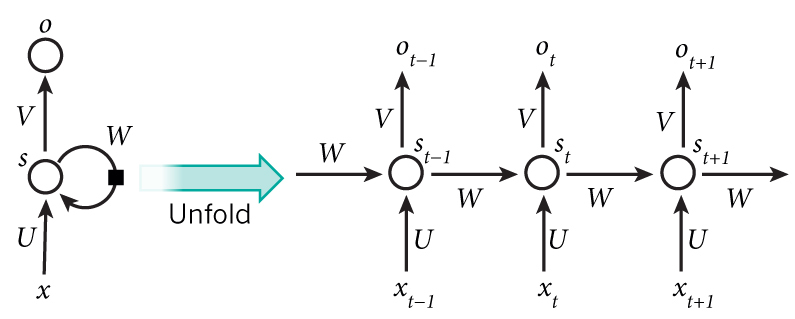
\includegraphics[width=0.7\textwidth]{graphs/rnn.png}
    \caption{Unfolded RNN cell $h$, across timesteps. $U$ and $V$ on the diagram are equivalent to $W_{h}$ and $U_{h}$ in Equation \ref{eq:rnns}. $W$ and $o_{t}$ represent the output generated from the hidden output $h_{t}$ \cite{RNN_diagram}.}
    \label{fig:rnn}
\end{figure}

Recurrent Neural Networks (RNNs) are a form of machine learning tasked with learning internal representations of sequential data first proposed by Rumelhart \textit{et al.} \cite{rnns} in 1986. RNNs introduced recurrent connections between neutrons, allowing them to retain information and capture contextual information from previous inputs. The ability to remember previous information made them particularly suitable for tasks involving sequential data such as language modeling, speech recognition and machine translation. By modelling dependencies between elements in a sequence, RNNs can effectively analyse the temporal dynamics of an input. The recurrent connections are described in Equation \ref{eq:rnns} below.

\begin{equation}
    \begin{gathered}
        h_{t} = \phi_{h}\left( W_{h}x_{t} + U_{h}h_{t-1} + b_{h} \right)
    \end{gathered}
    \label{eq:rnns}
\end{equation}

Where $h_{t}$ represents the hidden state at time step $t$ in the RNN. This captures the information learned from previous time steps and serves as a memory of past inputs. $\phi_{h}, W_{h}, U_{h}$ and $b_{h}$ represent the activation function and weight and bias matrices for the current cell $h$ of the model. The unrolling of a cell across multiple time steps can be seen in Figure \ref{fig:rnn}.

Traditional RNNs suffer from two primary challenges: vanishing gradients and limited memory capacity. When we train RNNs, the backpropagation algorithm involves computing gradients and propagating them back through time. However as the gradients are repeatedly multiplied through the recurrent connections, they can diminish exponentially over time leading to vanishing gradients. This challenge makes it harder for the model to capture long-term dependencies accurately as without strong gradient signals, the RNN struggles to propagate information across distant time steps, limiting its ability to learn meaningful representations from long sequences. The issue of limited memory capacity stems from the RNN's fixed-size internal memory, represented by the hidden state, meant to retain information from previous time steps. However, this memory limit can be insufficient to effectively capture complex dependencies in long sequences leading to a degradation in performance when attempting to retain information across distant time steps.

These limitations hinder the effectiveness of traditional RNNs in capturing long-term dependencies in sequential data. As a result, tasks that require modeling extensive context or handling long sequences, such as understanding complex language patterns or maintaining context in conversations, can pose significant challenges to RNN-based approaches. In recent years, advancements in NLP have seen a shift towards the use of Transformer-based architectures, which have emerged as a powerful alternative to RNNs. 

RNNs were a big step toward creating models which can understand temporal data such as the written text, however, due to the limitations mentioned, they are still not the answer to giving computers the ability to fully understand the written text. In the following sections, we will explore the Transformer model and its applications in NLP, highlighting its advantages over traditional RNN-based approaches and how they solve some of the limitations we face in RNNs.

\section{Transformers}

Transformers were first introduced by Vaswani \textit{et al.} \cite{transformer_paper} to effectively capture and leverage the relationships between elements in a sequence, with the main application being within the field of Natural Language Processing. They proposed a novel approach that relied on attention mechanisms to allow the model to attend to different sections of the input sequence to overcome the limitations of recurrent neural networks with the hope of overcoming the limitations of long-term dependencies found in previous models.

\subsection{Transformer Architecture}

The transformer model is composed of 6 identical layers of encoders and decoders. On the left side of Figure \ref{fig:transformer_arch} we can see the diagram for the encoder, consisting of two sublayers - a multi-head attention and a position-wise fully connected feed-forward network. The goal of the encoder is to take in the input and capture contextual information in order to create a meaningful representation of input tokens. This layer is repeated N times after which the output is passed through to the decoder which can be seen on the right portion of the figure. In addition to the two sub-layers found in the encoder, the decoder inserts a third layer, performing multi-head attention over the output of the encoder. The goal of the decoder is to generate an output sequence based on the encoded input representation. All layers also employ the use of residual connections and layer normalisation to facilitate the flow of information within each model and help combat issues such as vanishing or exploding gradients.

\begin{figure}[H]
    \centering
    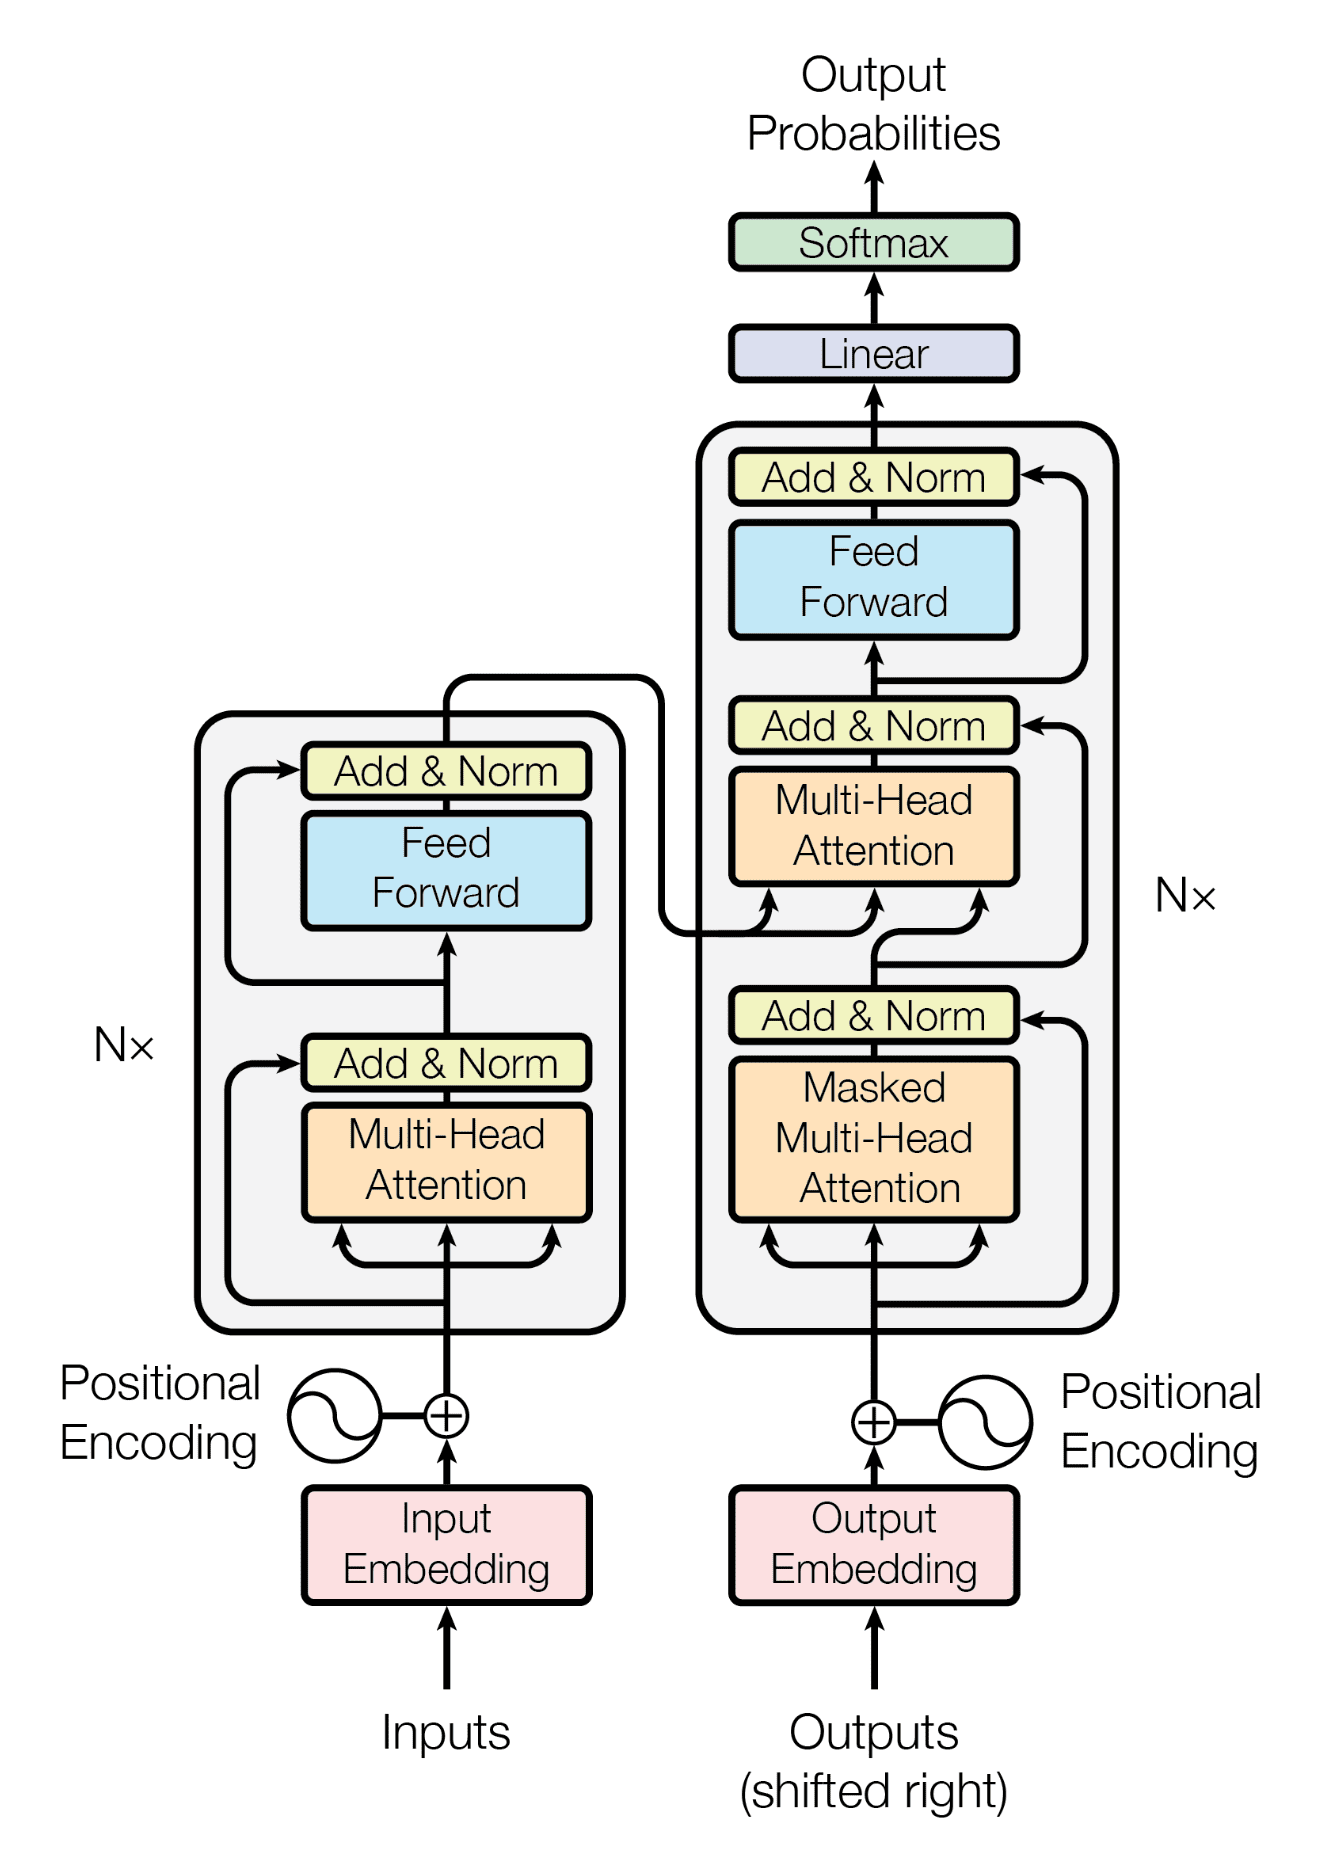
\includegraphics[width=0.5\textwidth]{graphs/transformer_architecture.png}
    \caption{Transformer Architecture as proposed by Vaswani \textit{et al.} \cite{transformer_paper}. It contains the encoder and decoder, mapping the route inputs take through the model}
    \label{fig:transformer_arch}
\end{figure}

\subsection{Multi-Head Attention}

Self-attention is a mechanism employed by Transformers to enable a sequence to attend to itself, capturing long and short-range dependencies and relationships among the tokens of the input. Self-attention is described as the combination of 3 different inputs: Queries ($Q$), Keys ($K$) and Values ($V$).

\begin{equation}
    \begin{gathered}
        \text{Attention}(Q,K,V) = softmax \left( \frac{QK^T}{\sqrt{d_k} } \right) V
    \end{gathered}
    \label{eq:self_attention}
\end{equation}

The value of $d_{k}$ represents the dimensionality of the matrix K and serves the purpose of normalising the attention weights and controlling the scale of the attention mechanism. In the encoder, the attention blocks are known as self-attending where $Q$, $K$, and $V$ are all set to be equal, where the values correspond to the outputs of the preceding layer. This symmetry in the self-attention mechanism promotes the capture of relationships and dependencies within the input sequence. As a result, each position in the sequence can attend to every other position, including itself, promoting a thorough understanding of the contextual connections throughout the sequence. In the decoder, a cross-attention block is introduced in which the $K$ and $V$ matrices are derived from the encoder's output while the query matrix, $Q$, is derived from the previous decoder layer's output. This allows the decoder to incorporate information from the encoder, aligning the input sequence with the relevant context during the decoding process.

Transformers introduced an update to the traditional self-attention by incorporating multi-head self-attention (MHA) \cite{mha_paper}, allowing the model to capture a more diverse range of information, learning multiple dependencies across the same input sequence. In MHA, the self-attention mechanism is applied multiple times in parallel, with different sets of learned matrices for each attention head. All outputs of the attention heads are then concatenated and transformed to generate the final output:

\begin{equation}
    \begin{gathered}
        \text{MultiHeadAttention}(Q,K,V) = \text{Concat}\left( A(Q_{1}, K_{1}, V_{1}), ...,  A(Q_{h}, K_{h}, V_{h})\right) W^{O}
    \end{gathered}
    \label{eq:mha}
\end{equation}

Where $Q_{i} = QW_{i}^{Q}, K_{i} = KW_{i}^{K}, V_{i} = VW_{i}^{V}, W^{O} \in \mathbb{R}^{hd_{k} \times d}$, $h$ is the number of heads per layer and $W^{O}$ is the learned weight matrix applied to the concatenation of attention outputs.

\subsection{Position-Wise Feed-Forward Network}

Each layer of the encoder and decoder also contains a fully connected feed-forward network consisting of two linear transformations with a ReLU activation between:

\begin{equation}
    \begin{gathered}
        \text{FFN}(x) = \max \left(0, xW_{1} + b_{1}\right)W_{2} + b_{2}
    \end{gathered}
    \label{eq:ffnn}
\end{equation}

Where $W_1 \in \mathbb{R}^{d_{model} \times d_{ff}}, W_2 \in \mathbb{R}^{d_{ff} \times d_{model}}$. In the original paper, $d_{model} = 512$ and $d_{ff} = 2048$.

Positional encodings are also added to the input embeddings to provide the model with information on the relative positions of tokens in the input. These allow the Transformer to capture the sequential order of tokens as the original self-attention mechanism itself does not possess any notion of token order. These encodings are represented as fixed-length vectors with the same dimensionality as the input embeddings. They are based on sine and cosine functions of different frequencies, following these functions:

\begin{equation}
    \begin{aligned}
        \text{PE}(\text{pos}, 2i)     & = \sin\left(\text{pos} / 10000^{(2i/d_{model})}\right) \\
        \text{PE}(\text{pos}, 2i + 1) & = \cos\left(\text{pos} / 10000^{(2i/d_{model})}\right)
    \end{aligned}
    \label{eq:pos_embedding}
\end{equation}

Where $i$ represents the $i$th dimension of the position $pos$ and $d_{model}$ represents the dimensionality of the input embeddings.

\section{BERT Model}
\label{sec:BERT}
After the introduction of the Transformer model, subsequent advancements led to the development of transformer-based models such as BERT (Bidirectional Encoder Representations from Transformers) \cite{BERT}, a language model created by Google. These models were designed to enhance the language model's ability to generalise across various tasks, including machine translation and text generation.

BERT was specifically designed to comprehend the contextual relationships between words in a given text, allowing it to analyse the context and understand the intended meaning. Consequently, it is well-suited for tasks such as detecting toxicity and hate in messages, as the context of a sentence plays a crucial role in determining its intent. Since its inception in 2018, BERT has seen notable variations, including RoBERTa (Robustly Optimized BERT Approach) and ALBERT (A Lite BERT). RoBERTa \cite{RoBERTa} was designed to be an upgrade on BERT, created by Facebook AI. Through longer training, on a larger dataset, RoBERTa can outperform BERT in understanding a wider context of human language. ALBERT \cite{AlBERT}, on the other hand, was designed to perform faster by massively reducing the number of parameters.

\subsection{BERT Architecture}

One of the significant advancements BERT creates is its incorporation of bidirectional context into the language representation. The original Transformer used self-attention mechanisms to understand relationships between different input tokens. However, it processed inputs in a unidirectional manner, either from left to right or vice versa. While this is an appropriate approach for many tasks, it falls short when a more comprehensive understanding of the input's context is necessary. BERT addresses this limitation by considering both the forward and backward context of each token during training, allowing it to capture more nuanced dependencies between words.

To achieve bidirectional context modeling, BERT utilises a technique called "Masked Language Modelling". This is a process in which some of the words in the input sentence are replaced by a masking token such as "\verb|[MASK]|". The model is then tasked with predicting the missing words, forcing the model to learn the meaning and representation between words in an input sequence. BERT applied this method by taking 15\% of the input tokens and applying one of three changes to them:

\begin{enumerate}[itemsep=0pt, topsep=1pt]
    \item 80\% of the tokens are replaced with the "\verb|[MASK]|" token to train the model at better handling incomplete inputs
    \item 10\% of the tokens are replaced with a random word from the corpus to train the model at better handling random noise
    \item 10\% of the tokens are left the same to help bias the representation into the actual observed word
\end{enumerate}

The tokenisation process proposed by Devlin \textit{et al.} \cite{BERT} is illustrated in Figure \ref{fig:bert}. The initial tokens, including special classification tokens such as \verb|[CLS]| and separator tokens such as \verb|[SEP]| are transformed into token embeddings. These token embeddings are then combined with segment embeddings, indicating which segment each token belongs to, and positional embeddings, which encode the token's position within the sequence.

This inclusion of segment embeddings is particularly useful for tasks that require multiple sentences or paragraphs as inputs as it allows BERT to differentiate between different segments of the input. This helps facilitate the capture of contextual relationships across sentence boundaries.

\begin{figure}[H]
    \centering
    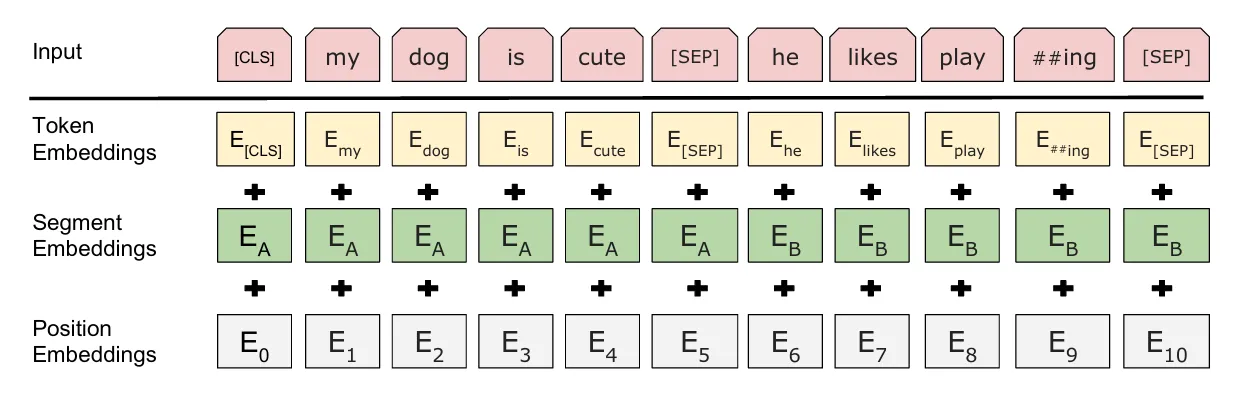
\includegraphics[width=0.8\textwidth]{graphs/bert.png}
    \caption{BERT input representation by Devlin \textit{et al.} \cite{BERT}. Input embeddings are the sum of token, segmentation and position embeddings.}
    \label{fig:bert}
\end{figure}

Another notable aspect of BERT is the use of a pre-training and fine-tuning paradigm in which the model is first pre-trained on a large corpus of unlabeled text, utilising both masked language modeling objectives and next sentence prediction. The pre-training phase allows BERT to learn general language representations from vast amounts of unlabeled data, freely available on the internet. Once pre-training has been completed, the model can be fine-tuned on specific downstream tasks by adding task-specific layers and fine-tuning with labeled data. This process uses the general language understanding BERT has learned from pre-training to the specific requirement of the task, resulting in highly performant models across a vast range of NLP tasks.

\subsection{Sentiment Analysis}

We are interested in the use of Transformers for text classification through the fine-tuning of pre-trained language models. One of the downstream tasks proposed by Devlin \textit{et al.} meant to evaluate the ability of BERT was to create a text classification model. In their model a special \verb|[CLS]| token was used to produce a corresponding output $C$ that was fed into a separate classification layer to obtain the sentence logits.

\begin{equation}
    \begin{gathered}
        y = \phi\left( W_{c}C+b_{c} \right)
    \end{gathered}
    \label{eq:bert_classification}
\end{equation}

Where $W_{c}$ and $b_{c}$ are learned weights and biases used for classification. $y \in \mathbb{R}^c$ where $c \in \mathbb{N}$ is the number of class labels in the multi-label classification. The authors then used the Stanford Sentiment Treebank (SST) dataset to train and benchmark BERT's ability to classify sentences into different sentimental categories, achieving a final accuracy of \textbf{92.7\%}. We can utilise this same process to create a text classification model capable of detecting toxic text and classifying it into one of many labels.

\subsection{RoBERTa}

RoBERTa, introduced by Liu \textit{et al.} \cite{RoBERTa}, is a variant of the BERT architecture that aims to enhance its performance and address certain limitations. RoBERTa builds upon the success of BERT but introduces additional modifications to improve its pre-training process.

One notable difference in RoBERTa is the use of larger batch sizes during pre-training. By increasing the batch size, RoBERTa benefits from more diverse and varied sentence pairs, resulting in improved generalisation capabilities. Additionally, RoBERTa leverages a longer training duration, which enables it to achieve even better performance compared to BERT.

Furthermore, RoBERTa removes the next sentence prediction (NSP) task from the pre-training process. This change allows the model to focus solely on the masked language modeling (MLM) task, resulting in better utilisation of the training data and more effective learning of contextual representations.

Overall, RoBERTa improves upon BERT's pre-training methodology and achieves state-of-the-art performance on various downstream tasks. With its larger batch sizes, longer training duration, and larger architecture, RoBERTa demonstrates enhanced capability in capturing deep contextual understanding and achieving robustness in natural language processing tasks.

\subsection{AlBERT}

AlBERT, produced by Lan \textit{et al.} \cite{AlBERT}, is a variation of the BERT architecture that addresses several limitations of the original model. One key improvement is the introduction of parameter sharing across layers, which significantly reduces the model's memory footprint and enhances its efficiency and scalability compared to BERT. This makes AlBERT particularly suitable for deploying models in resource-constrained environments, such as mobile devices. In terms of parameter count, while BERT has around 110 million parameters (and RoBERTa has 125 million), AlBERT achieves comparable performance with only 11 million parameters.

However, AlBERT does come with certain trade-offs. Due to the sharing of parameters, the capacity for individual layer-specific learning is reduced. This limitation can impact the model's ability to capture fine-grained features at each layer, potentially affecting its performance on tasks that require deep contextual understanding. Additionally, AlBERT may not achieve the same level of performance as BERT or other variations, such as RoBERTa, on certain complex language understanding tasks.

Despite these limitations, AlBERT presents a valuable alternative, especially in scenarios where memory efficiency and scalability are critical factors. Its reduced parameter count and improved efficiency make it well-suited for deployment in resource-limited settings, where maintaining a balance between model capability and resource constraints is of utmost importance.

\section{Application}

In this chapter, we have explored the vast potential of artificial intelligence in comprehending written text and making informed decisions, particularly in tasks like sentiment analysis. We delved into the advancements and constraints associated with RNN structures, paving the way for our choice of the Transformer-based architecture of AlBERT. By adopting this powerful framework, we aim to develop a sentiment analysis model that is not only highly accurate but also optimized for client-side deployment on mobile devices.